\documentclass[crop,tikz]{standalone}

\usepackage{tikz}
\usepackage{anyfontsize}

\usetikzlibrary{matrix}
\usetikzlibrary{arrows.meta}
\begin{document}

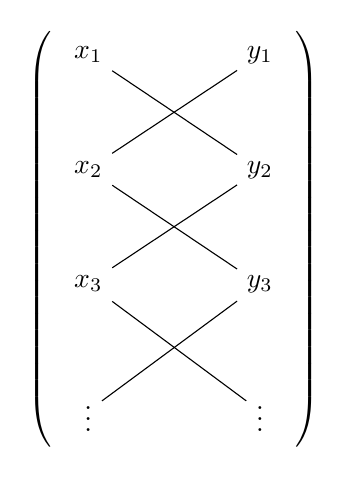
\begin{tikzpicture}
\matrix (M)[matrix of math nodes,row sep=1cm,column sep=16mm,left delimiter=(,right delimiter=)]{
x_1 & y_1 \\ x_2 & y_2 \\ x_3 & y_3 \\ \vdots & \vdots\\
};
\draw (M-1-1)--(M-2-2);
\draw (M-1-2)--(M-2-1);
\draw (M-2-1)--(M-3-2);
\draw (M-2-2)--(M-3-1);
\draw (M-3-1)--(M-4-2);
\draw (M-3-2)--(M-4-1);

\end{tikzpicture}
\end{document}